% 本文件为原模板的正文填充区。
\section*{实验五：异常处理与脏数据健壮处理}

\section{实验目的}
\begin{enumerate}
  \item 掌握 \texttt{try-catch-finally} 与 \texttt{throw/throws} 的用法。
  \item 定义并使用自定义受检异常，准确描述数据错误原因。
  \item 对脏数据、缺失值和格式错误逐行处理，使数据加载过程能够继续执行。
\end{enumerate}

\section{实验环境}
操作系统为 macOS，Java 环境为 Eclipse Temurin OpenJDK 17.0.20.1，
源文件编码为 UTF-8，课程规定实验学时为 3 学时。报告使用课程提供的
\texttt{ZAFUReport} 原始模板。

\section{实验内容与步骤}
\subsection{任务一：捕获常见异常}
在 \texttt{ExceptionDemo.run()} 中分别构造并捕获以下四种异常：
\begin{enumerate}
  \item 对字符串 \texttt{abc} 调用 \texttt{Integer.parseInt}，捕获 \texttt{NumberFormatException}。
  \item 访问长度为 2 的数组的第 3 个位置，捕获 \texttt{ArrayIndexOutOfBoundsException}。
  \item 对整数执行除以零，捕获 \texttt{ArithmeticException}。
  \item 对 \texttt{null} 引用调用方法，捕获 \texttt{NullPointerException}。
\end{enumerate}
这些异常分别处理，之后程序继续运行。方法 \texttt{returnWithFinally()} 在
\texttt{try} 中准备返回，\texttt{finally} 在方法实际返回之前输出提示；
主程序随后打印返回值，从输出顺序可验证这一行为。
\texttt{finally} 通常会执行，但 JVM 被强制终止等情况不保证执行。

\subsection{任务二：自定义异常}
\texttt{InvalidDataException} 继承 \texttt{Exception}，属于受检异常。
\texttt{parseLine} 在方法签名中用 \texttt{throws} 声明它，发现错误时使用
\texttt{throw} 抛出。异常使用枚举保存稳定的错误类别，并保留可读描述；
数字解析失败时保存原始异常作为原因。错误类型包含字段缺失、字段数量错误、
编号非数字或超出 \texttt{long} 范围、分数非数字和分数越界。
编号转换与分数转换分别捕获，避免把错误编号误报成分数非数字。

输入约定为简单的 \texttt{编号,姓名,分数} 三字段文本；不支持带引号的逗号或跨行 CSV 字段。
使用 \texttt{split(",", -1)} 保留尾部空字段，再检查空值、字段数量和分数范围。
分数使用 \texttt{BigInteger} 解析，以便将超出整数范围的纯数字仍归为“分数越界”，
而非误报为“分数非数字”。分数只接受 0 至 100 的整数。

\subsection{任务三：健壮的数据加载}
\texttt{loadData(String[] lines)} 逐行调用 \texttt{parseLine}，成功记录加入列表；
发生 \texttt{InvalidDataException} 时保存原行、行号及错误类别，跳过该行并继续解析。
使用 \texttt{EnumMap} 按错误类别计数；结果对象提供不可修改的记录、错误列表和统计映射。
空数组产生空结果，单行 \texttt{null} 被视为字段缺失；输入数组本身为 \texttt{null}
则明确抛出 \texttt{NullPointerException}，以区分调用错误与单条脏数据。

\subsection{实验源码}
以下为各任务的完整 Java 源码，独立源文件随报告工程提交。
\subsubsection{成绩记录和自定义异常}
\lstinputlisting[language=java]{DataRecord.java}
\lstinputlisting[language=java]{InvalidDataException.java}
\subsubsection{常见异常与 finally}
\lstinputlisting[language=java]{ExceptionDemo.java}
\subsubsection{逐行加载及主程序}
\lstinputlisting[language=java]{RobustLoader.java}

\section{实验结果与分析}
使用 JDK 17 执行 \texttt{./run.sh}，退出状态为 0。图~\ref{fig:run} 是浏览器
展示实际程序输出的截图；原始输出保存在“运行结果.txt”。
\begin{figure}[htbp]
  \centering
  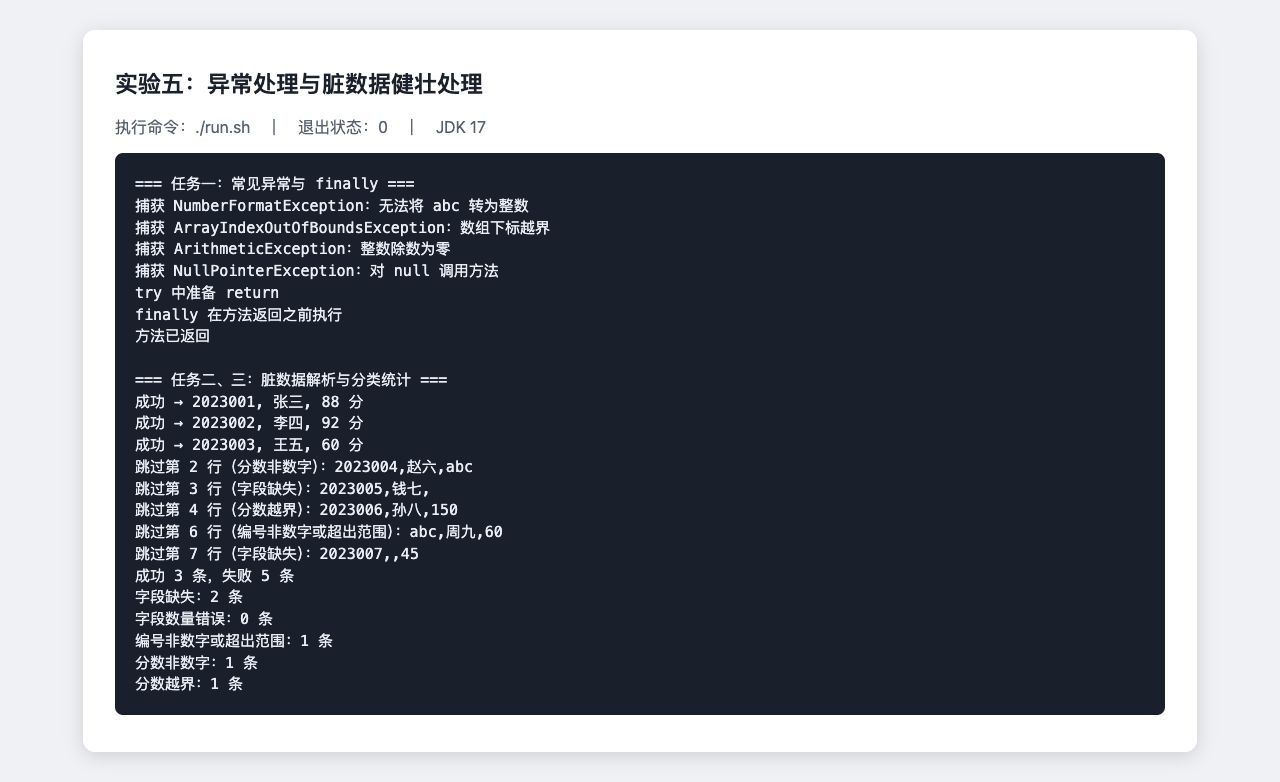
\includegraphics[width=\textwidth]{figure/运行结果截图.png}
  \caption{程序实际运行结果：异常处理、跳过脏数据与分类统计}
  \label{fig:run}
\end{figure}

示例共 8 行，成功 3 条、失败 5 条，分类统计为：字段缺失 2 条、字段数量错误 0 条、
编号非数字或超出范围 1 条、分数非数字 1 条、分数越界 1 条，各类失败数量之和为 5。
虽然第 2 至 4 行包含不同错误，后面的合法记录仍被成功加载。
另有 23 项独立检查，覆盖 0 和 100 边界、缺失字段、额外字段、错误编号、极大分数、
空数组、不可变结果以及 \texttt{finally} 的执行顺序，检查全部通过。

\section{思考题}
\subsection{RuntimeException 与受检异常是否强制处理？}
\texttt{RuntimeException} 及其子类属于非受检异常，编译器不强制调用者捕获或声明。
\texttt{IOException} 等受检异常若可能从方法中抛出，通常必须在方法内捕获处理，
或通过 \texttt{throws} 声明交由调用者处理；重写方法还需遵循受检异常的声明限制。
本实验的 \texttt{InvalidDataException} 为受检异常，\texttt{parseLine} 声明抛出，
\texttt{loadData} 在每一行的循环中捕获。

\subsection{finally 的典型用途是什么？}
\texttt{finally} 常用于释放资源和清理状态，因为无论正常执行、发生异常，
还是在 \texttt{try} 或 \texttt{catch} 中返回，通常都会执行清理代码。
将关闭操作放在 \texttt{finally} 可以减少异常路径遗漏关闭资源的情况。
对实现 \texttt{AutoCloseable} 的资源，优先使用 \texttt{try-with-resources}，
它会在退出作用域时自动关闭，并能保留主异常与关闭时产生的受抑制异常。
断电、进程被强制终止或 JVM 直接退出等情况不保证执行 \texttt{finally}。

\subsection{catch (Exception e) 有什么隐患？}
宽泛捕获可能把程序缺陷（如空指针）与预期的数据错误混在一起，隐藏故障、
误报成功或使程序带着错误状态继续运行；还可能丢失异常上下文或需要特殊处理的中断信号。
应优先捕获能够合理处理的具体异常，保留原因和必要信息；
对无法处理的异常应继续抛出，若捕获 \texttt{InterruptedException} 后不能传播，
应按任务语义恢复中断状态。

\section{实验小结}
本实验完成常见异常捕获、自定义受检异常及逐行脏数据处理，验证了返回前
\texttt{finally} 的执行顺序，并通过分类计数和边界检查确认后续合法数据能够继续加载。

GitHub 仓库地址：\url{https://github.com/alerk2005-sketch/DataInsight}。
实验源码、运行截图、输出及验证材料随工程提交。
